\chapter{EL EJE SINTÉTICO: DATASET CON GROUND-TRUTH, PLAUSIBILIDAD Y ANÁLISIS ESTADÍSTICO}

El Capítulo 4 mostró que el \textit{Elliptic Dataset}, pese a su valor como referente de datos reales, impone un límite estructural, ya que su dispersión extrema impide medir la plausibilidad de las explicaciones y su desplazamiento temporal provoca el colapso del rendimiento en test. Este capítulo introduce un segundo eje experimental que responde de forma directa a esas limitaciones, un grafo sintético construido con \textit{ground-truth} de tipología que hace medible aquello que Elliptic no permite. El capítulo justifica primero por qué este eje es necesario y por qué no constituye un dataset ajustado a conveniencia, describe después la construcción del grafo y sus tipologías, y presenta a continuación los resultados de la matriz factorial completa. La parte final del capítulo despliega el análisis estadístico de robustez, argumenta por qué se aplican determinadas pruebas y expone los tres hallazgos centrales, a saber la superioridad de PGExplainer en plausibilidad de aristas, la ausencia de un puente entre estabilidad y plausibilidad, y la disociación entre plausibilidad y fidelidad.

\section{Por qué se Construye un Grafo Sintético}

La afirmación de que una explicación es plausible exige comparar el subgrafo o las features que el explicador señala como relevantes con un patrón de referencia que se sepa verdadero. En el \textit{Elliptic Dataset} ese patrón de referencia no existe, por dos razones que se refuerzan mutuamente. La primera es que sus 166 features están anonimizadas, de modo que se desconoce qué atributo corresponde a qué propiedad de la transacción y no puede afirmarse que una feature señalada sea la correcta. La segunda es que los vecindarios ilícitos son de apenas dos o tres nodos, según se documentó en el Capítulo 4, lo que deja sin estructura suficiente a cualquier explicación a nivel de subgrafo. Por estas dos razones, la plausibilidad de las explicaciones no es una magnitud medible en Elliptic, con independencia de la calidad del explicador utilizado.

El grafo sintético no reemplaza al \textit{Elliptic Dataset}, sino que lo complementa, y esta distinción es esencial para entender el diseño de la tesis. El eje Elliptic aporta validez externa, puesto que se trata de datos reales de Bitcoin con todo su ruido, su desbalance y su desplazamiento temporal, condiciones que ningún grafo sintético reproduce con fidelidad. El eje sintético aporta validez interna para la afirmación de plausibilidad, ya que ofrece control total sobre la construcción del grafo y un \textit{ground-truth} explícito de qué aristas y qué features definen cada tipología de lavado. La combinación de ambos ejes permite sostener conclusiones que ninguno de los dos podría sostener por separado, un rendimiento sobre datos reales y una evaluación de plausibilidad sobre datos controlados.

Conviene anticiparse a una objeción legítima, la de que un grafo construido a la medida podría diseñarse para producir el resultado deseado. Esta objeción se responde de dos maneras. En primer lugar, el uso de grafos sintéticos con \textit{ground-truth} es una práctica establecida en la evaluación de explicadores de GNN, dado que GNNExplainer se validó originalmente sobre grafos con motivos inyectados y los estudios rigurosos de evaluación de explicabilidad recurren a referencias sintéticas precisamente porque los datos reales carecen de \textit{ground-truth} \cite{Ying2019Gnnexplainer:Networks, Agarwal2022ProbingMethods}. En segundo lugar, y de forma más contundente, los resultados obtenidos son incómodos y no convenientes, ya que el estudio encuentra un puente nulo entre estabilidad y plausibilidad y una tensión difícil de explicar entre plausibilidad y fidelidad. Un dataset ajustado a conveniencia habría producido una correlación limpia y positiva que confirmara la hipótesis de partida, mientras que el grafo utilizado produjo un no resultado honesto y una disociación que complica la interpretación, lo que constituye la mejor prueba de que no se ajustó a un desenlace prefijado.

\section{Construcción del Grafo Sintético y sus Tipologías}

El grafo sintético consta de alrededor de 9.500 nodos, de los cuales cerca de 1.530 son ilícitos, conectados por unas 31.000 aristas. Sobre un fondo de cuentas lícitas con transacciones dispersas se inyectan cuatro tipologías de lavado con \textit{ground-truth} por nodo y por arista, a saber \textit{structuring}, que reparte fondos de un origen hacia muchos intermediarios en montos pequeños, \textit{layering}, que encadena transferencias a lo largo de una cadena de cuentas, y las variantes \textit{fan-in} y \textit{fan-out}, que concentran fondos desde muchas cuentas hacia una o los distribuyen desde una hacia muchas. Cada nodo y cada arista de patrón queda etiquetado con la tipología a la que pertenece, lo que constituye la referencia contra la cual se mide la plausibilidad de las explicaciones.

Tres decisiones de construcción resultan determinantes para que el grafo sea a la vez realista y evaluable. La primera es la simetrización de las aristas, necesaria porque con aristas dirigidas el campo receptivo de un nodo de patrón cae a una mediana de dos nodos, la misma dispersión que impide medir plausibilidad en Elliptic, mientras que la simetrización eleva esa mediana a cerca de veintinueve nodos y hace medible la plausibilidad a nivel de subgrafo. La segunda es la incorporación de aristas distractoras, que conectan cada nodo de patrón con el fondo lícito, de modo que el vecindario mezcle aristas de patrón con ruido y solo un explicador que señale correctamente el patrón obtenga una plausibilidad alta, evitando que cualquier selección acierte de forma trivial. La tercera es la atenuación de la firma de features, ya que cada tipología eleva una feature específica en sus nodos, pero con una magnitud moderada que impide que la plausibilidad de features resulte trivialmente perfecta, un ajuste que se introdujo tras verificar que una firma demasiado marcada volvía la tarea demasiado fácil.

Antes de emplear el grafo en los experimentos, se verificó que la simetrización lograra su objetivo, midiendo el tamaño del campo receptivo de los nodos de tipología. La mediana resultante, cercana a veintinueve nodos, confirma que el subgrafo receptivo de un nodo de patrón contiene estructura suficiente para que una explicación a nivel de subgrafo sea evaluable, en contraste con los dos nodos de mediana del \textit{Elliptic Dataset}. Esta verificación es esencial, ya que sin ella el eje sintético reproduciría la misma limitación que motivó su construcción. El generador fija además el número de patrones de cada tipología para que ninguna quede subrepresentada en el muestreo de nodos a explicar, un ajuste que se introdujo tras observar que las cadenas de \textit{layering}, más cortas, quedaban con pocos ejemplos frente a las demás tipologías.

Cada tipología se define no solo por su estructura de aristas sino también por una feature de firma que se eleva en sus nodos, lo que permite medir la plausibilidad tanto a nivel de aristas como de features. La existencia de esta doble referencia, estructural y de atributos, es lo que convierte al grafo sintético en un banco de pruebas completo para la plausibilidad, dado que un explicador puede acertar en las aristas y fallar en las features, o a la inversa. Las aristas distractoras, por su parte, cumplen la función de evitar que la tarea sea trivial, ya que sin ellas cualquier selección de aristas dentro del subgrafo de patrón acertaría por construcción, y la plausibilidad dejaría de discriminar entre un explicador competente y uno que seleccionara aristas al azar.

\section{Resultados de la Matriz Factorial}

La matriz factorial sintética cruza las cuatro arquitecturas, los cinco escenarios de desbalance, las tres estrategias de balanceo y los tres explicadores, y da lugar a 180 celdas de resultado. La Figura \ref{fig:heatmap} resume el comportamiento de cada explicador a través de las cuatro métricas principales, y permite apreciar de un vistazo que ningún explicador domina en todas ellas. La lectura por columnas revela un patrón consistente, cada explicador destaca en una dimensión y se queda atrás en otra, lo que anticipa la ausencia de un método uniformemente superior. Este panorama contrasta con Elliptic, donde la dispersión impedía siquiera calcular la mayoría de estas métricas.

\begin{figure}[htbp]
    \centering
    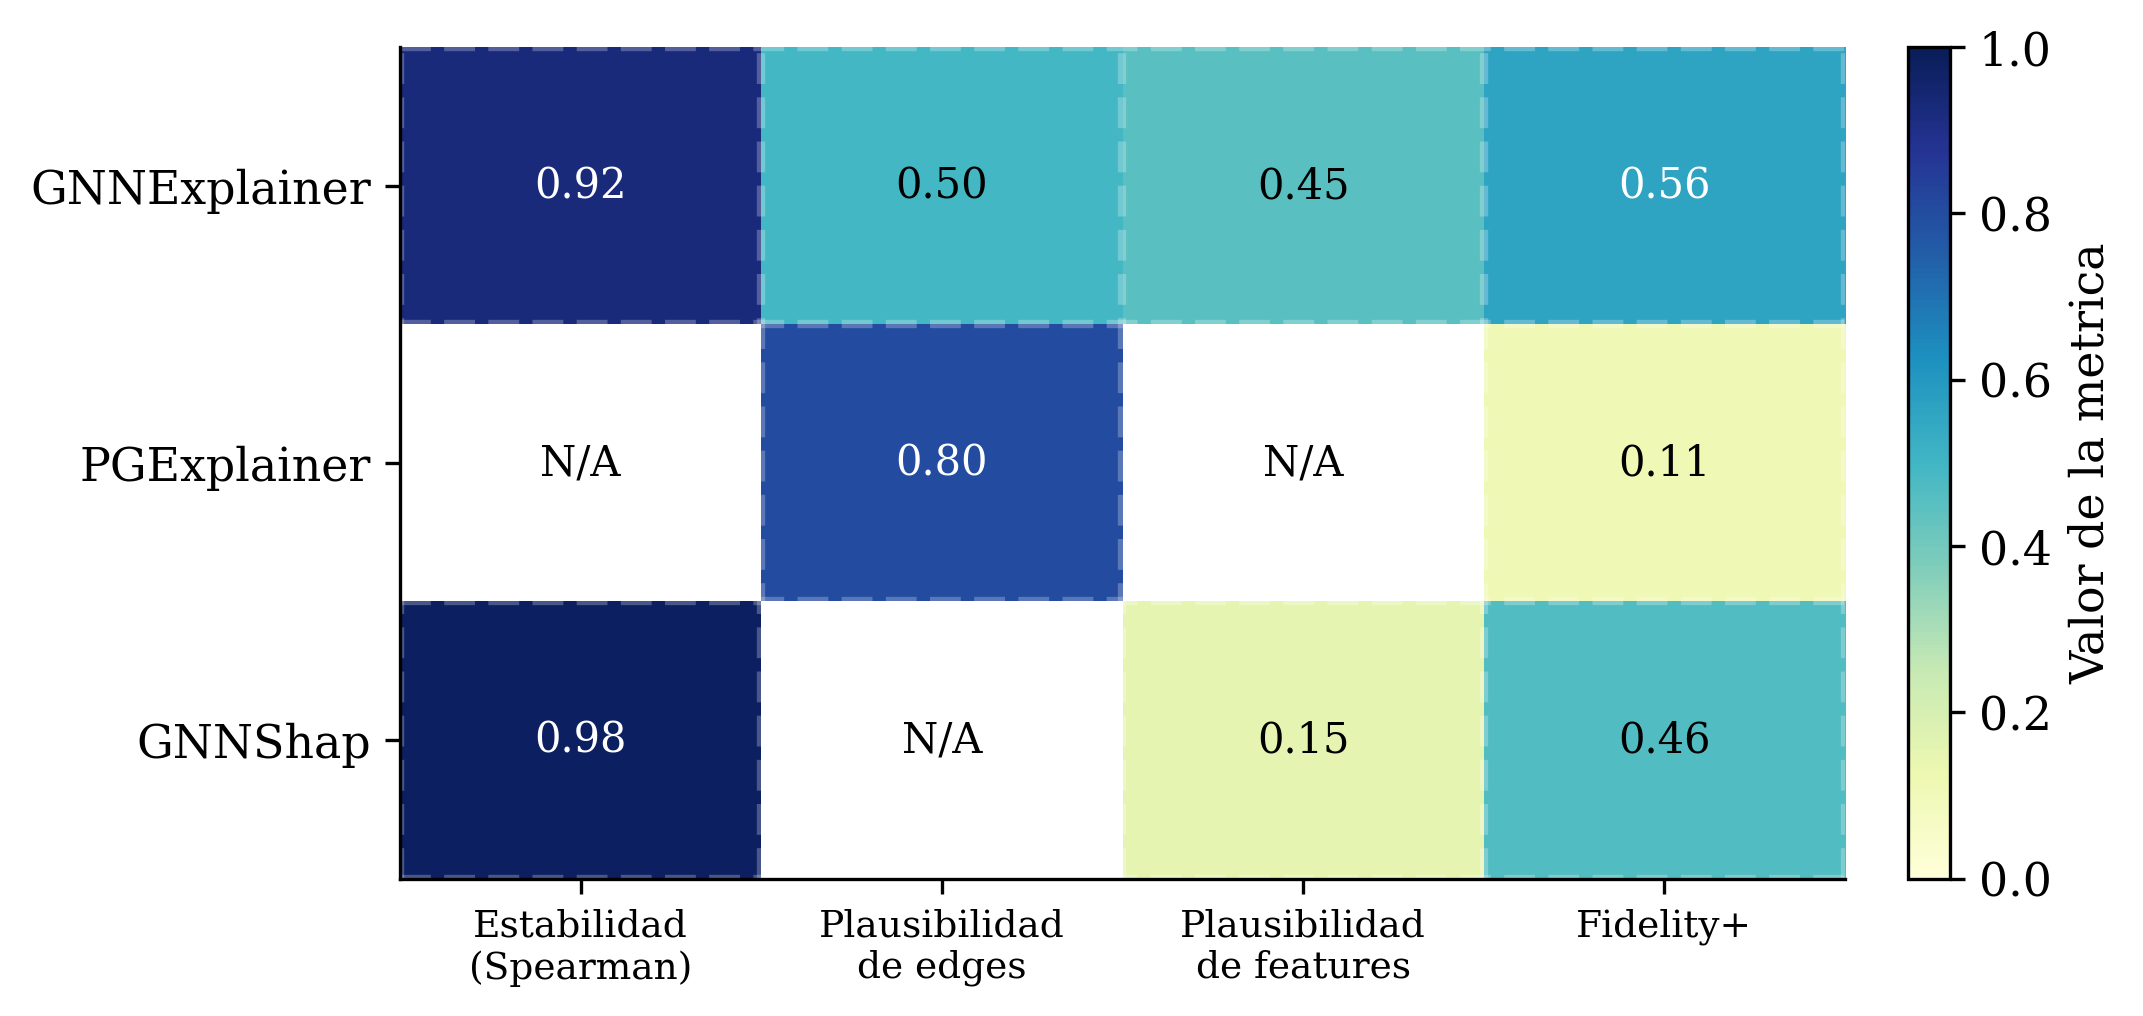
\includegraphics[width=0.95\textwidth]{chapter_5/images_ch5/heatmap_factorial.png}
    \caption{Comportamiento de los tres explicadores a través de cuatro métricas sobre el grafo sintético, promediado en la matriz factorial. Las celdas marcadas como N/A corresponden a métricas que un explicador no produce por diseño, como la estabilidad de PGExplainer, que es determinista tras entrenar, o la plausibilidad de aristas de GNNShap, que solo pondera features.}
    \label{fig:heatmap}
\end{figure}

En cuanto a la estabilidad, medida como la correlación de Spearman entre rankings de features, GNNShap resulta el más estable con un valor cercano a 0,977, por encima de GNNExplainer, que alcanza alrededor de 0,924. PGExplainer, por ser determinista una vez entrenado su modelo paramétrico, no admite una medida de estabilidad de este tipo, de modo que su celda se reporta como no aplicable. La estabilidad por arquitectura muestra un fenómeno digno de atención, ya que sobre el grafo denso GCN y GAT encabezan la estabilidad con valores cercanos a 0,965 y 0,960, con GraphSAGE y TAGCN por debajo, en torno a 0,889 y 0,886. Este orden coincide con el que arroja Elliptic una vez corregida la métrica de estabilidad, donde GCN y GAT también figuran a la cabeza, de modo que el orden de estabilidad entre arquitecturas resulta concordante entre ambos regímenes de densidad y ninguna arquitectura domina en términos absolutos. La Figura \ref{fig:contraste} contrasta directamente la estabilidad de GNNExplainer por arquitectura entre el régimen disperso de Elliptic y el régimen denso del grafo sintético, y hace visible la concordancia del orden.

\begin{figure}[htbp]
    \centering
    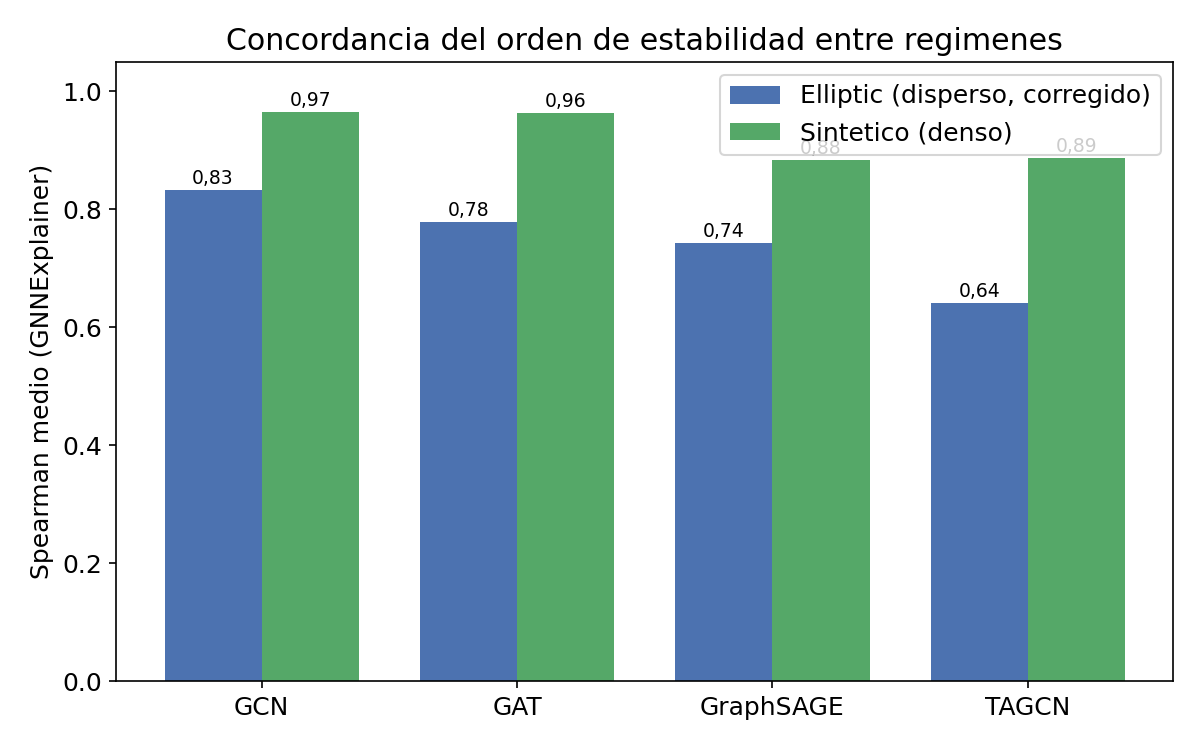
\includegraphics[width=0.85\textwidth]{chapter_5/images_ch5/contraste_regimen.png}
    \caption{Estabilidad de GNNExplainer por arquitectura en los dos regímenes de densidad. Con la métrica corregida, GCN y GAT encabezan la estabilidad tanto en el grafo disperso de Elliptic como en el grafo denso sintético, lo que evidencia que el orden de estabilidad es concordante entre regímenes y que GAT y GCN son las arquitecturas más estables con relativa independencia de la densidad.}
    \label{fig:contraste}
\end{figure}

La concordancia del orden de estabilidad entre los dos regímenes es un resultado con implicaciones conceptuales. Tanto en Elliptic, donde los vecindarios son minúsculos, como en el grafo denso sintético, GCN y GAT encabezan la estabilidad de las explicaciones, mientras que GraphSAGE y TAGCN quedan por debajo. La correlación de rangos de Spearman entre el orden de las cuatro arquitecturas en ambos regímenes cuantifica esta concordancia, ya que asciende a +0,80 con la métrica corregida, frente a -0,20 con la métrica defectuosa anterior, de modo que la reparación transforma una aparente inversión en una concordancia clara entre regímenes de densidad. Esto sugiere que la estabilidad de las explicaciones responde más al mecanismo de agregación de cada arquitectura que a la densidad del grafo sobre el que opera. Una recomendación de arquitectura orientada a la estabilidad, por tanto, parece transferirse entre regímenes de densidad distintos, si bien el reducido soporte de configuraciones con calidad garantizada en Elliptic obliga a confirmar esa transferencia con más datos antes de elevarla a regla general.

La plausibilidad revela el resultado más llamativo del eje sintético. En la plausibilidad de aristas, que mide cuán bien recupera el explicador las aristas de la tipología, PGExplainer alcanza un valor cercano a 0,801, muy por encima del 0,495 de GNNExplainer, mientras que GNNShap no produce máscara de aristas y queda fuera de esta comparación. En la plausibilidad de features, en cambio, GNNExplainer lidera con alrededor de 0,453 frente al 0,150 de GNNShap, y PGExplainer no genera un ranking de features. La fidelidad positiva, que mide cuánto cae la predicción al retirar los elementos que el explicador considera importantes, ordena a los tres métodos de otra manera, con GNNExplainer a la cabeza en torno a 0,561, GNNShap en 0,465 y PGExplainer muy por debajo, en valores de 0,110. Adicionalmente, la concentración de las atribuciones de GNNShap, medida contra el \textit{ground-truth}, alcanza un valor de 0,947, lo que ofrece una referencia cuantitativa para una métrica que en la literatura previa había quedado sin fundamento verificable. El detalle numérico completo por arquitectura y explicador se recoge en la Tabla \ref{tab:synth-factorial}, que confirma que ningún explicador domina simultáneamente en las cuatro métricas.

\begin{table}[htbp]
\centering
\renewcommand{\arraystretch}{1.3}
\small
\begin{tabular}{ll cccc}
\toprule
\textbf{Arquitectura} & \textbf{Explicador} & \textbf{Estab.} & \textbf{Plaus. aristas} & \textbf{Plaus. feat.} & \textbf{Fidelity+} \\
\midrule
GraphSAGE & GNNExplainer & 0,89 & 0,49 & 0,41 & 0,63 \\
GraphSAGE & PGExplainer & n/d & 0,92 & n/d & 0,13 \\
GraphSAGE & GNNShap & 0,97 & n/d & 0,19 & 0,55 \\
\midrule
GAT & GNNExplainer & 0,96 & 0,54 & 0,42 & 0,52 \\
GAT & PGExplainer & n/d & 0,68 & n/d & 0,12 \\
GAT & GNNShap & 0,97 & n/d & 0,18 & 0,43 \\
\midrule
GCN & GNNExplainer & 0,96 & 0,52 & 0,62 & 0,54 \\
GCN & PGExplainer & n/d & 0,73 & n/d & 0,12 \\
GCN & GNNShap & 0,99 & n/d & 0,15 & 0,51 \\
\midrule
TAGCN & GNNExplainer & 0,89 & 0,43 & 0,38 & 0,55 \\
TAGCN & PGExplainer & n/d & 0,86 & n/d & 0,07 \\
TAGCN & GNNShap & 0,97 & n/d & 0,09 & 0,37 \\
\bottomrule
\end{tabular}
\caption{Resultados de la matriz factorial sintetica por arquitectura y explicador (media sobre 3 semillas de modelo, grafo g0). Los valores n/d corresponden a metricas que un explicador no produce por diseno. Fidelity+ se calcula con la definicion manual uniforme (caida de probabilidad al retirar el top-k) para los tres explicadores. PGExplainer domina la plausibilidad de aristas, GNNExplainer la de features y la fidelidad, y GNNShap la estabilidad.}
\label{tab:synth-factorial}
\end{table}


Un resultado del eje sintético merece destacarse por su contraste con el Capítulo 4. Mientras que en Elliptic PGExplainer degeneraba de forma casi universal y producía una correlación nula, sobre el grafo denso PGExplainer no solo funciona, sino que se convierte en el explicador más plausible en aristas. Este contraste responde una pregunta metodológica que Elliptic dejaba abierta, la de si la degeneración de PGExplainer era un defecto del método o una consecuencia de la dispersión del dato. La evidencia del eje sintético indica claramente lo segundo, ya que con estructura de subgrafo suficiente PGExplainer recupera el patrón mejor que cualquier otro método, de modo que su fracaso en Elliptic se atribuye a la dispersión y no a una limitación intrínseca del explicador.

\section{Análisis Estadístico de Robustez}

Afirmar que una diferencia entre arquitecturas o entre explicadores es real exige separar la señal del ruido de una única inicialización, y la matriz factorial descrita hasta aquí entrenaba un solo modelo por celda, lo que no permitía esa separación. Para dotar de potencia inferencial al análisis, cada celda se replicó con tres semillas de modelo distintas, que producen entrenamientos independientes sobre los mismos datos, de manera que la variación entre semillas cuantifica cuánto de un resultado es atribuible al azar del entrenamiento. Esta replicación eleva la matriz a 540 filas sobre el grafo principal y se complementa con dos grafos adicionales generados con semillas distintas, para verificar que los hallazgos no dependen de una realización particular del generador. La dispersión entre semillas resultó muy baja, con una desviación típica de la correlación de Spearman media de apenas 0,007, lo que indica que los resultados son altamente reproducibles.

Esta baja dispersión tiene una lectura que va más allá de la reproducibilidad técnica. Un valor de estabilidad que apenas varía entre entrenamientos independientes indica que la propiedad medida es del método y del dato, y no de una inicialización afortunada, lo que otorga a las comparaciones entre explicadores una base firme. Sin esta verificación, cualquier diferencia observada entre dos explicadores podría atribuirse al azar de un único entrenamiento, y las conclusiones carecerían de respaldo. La replicación por semillas de modelo es, por tanto, lo que transforma un conjunto de observaciones en evidencia sobre la que se pueden sostener afirmaciones con una medida explícita de confianza.

Un control interno confirma que esta extensión es fiel al análisis original. El corte de la matriz correspondiente a la primera semilla reproduce con exactitud los valores de la matriz factorial de una sola corrida, lo que demuestra que la replicación añade réplicas sin alterar el procedimiento subyacente. Sobre esta base replicada se aplican las pruebas estadísticas introducidas en el Capítulo 3, elegidas en función de la naturaleza de las métricas. Puesto que las métricas de estabilidad y plausibilidad viven en el intervalo de cero a uno y no cumplen el supuesto de normalidad, la prueba principal para comparar factores es la de Kruskal-Wallis, acompañada del tamaño de efecto eta cuadrado, mientras que la comparación pareada entre dos explicadores recurre a la prueba de Wilcoxon de rangos con signo.

El análisis de factores arroja un resultado nítido, el explicador es el factor que más determina el comportamiento de las explicaciones. La Tabla \ref{tab:synth-stats} recoge la prueba de Kruskal-Wallis y el tamaño de efecto eta cuadrado de cada factor sobre cada métrica, y muestra que el explicador domina la estabilidad con un valor de 0,36, la plausibilidad de aristas con 0,64 y la plausibilidad de features con 0,45, cifras que corresponden a efectos grandes. La arquitectura ejerce un efecto grande únicamente sobre la estabilidad, con un valor de 0,24, y un efecto pequeño sobre las demás métricas. El balanceo, en cambio, resulta prácticamente irrelevante para la calidad de las explicaciones, con valores de eta cuadrado inferiores a 0,02 en todas las métricas, un hallazgo con implicaciones prácticas directas, ya que sugiere que la elección de la estrategia de balanceo apenas afecta a la plausibilidad o la estabilidad de las explicaciones obtenidas. La Figura \ref{fig:balanceo} ilustra esta irrelevancia, al mostrar que las tres estrategias de balanceo producen valores casi idénticos en las tres métricas principales.

\begin{figure}[htbp]
    \centering
    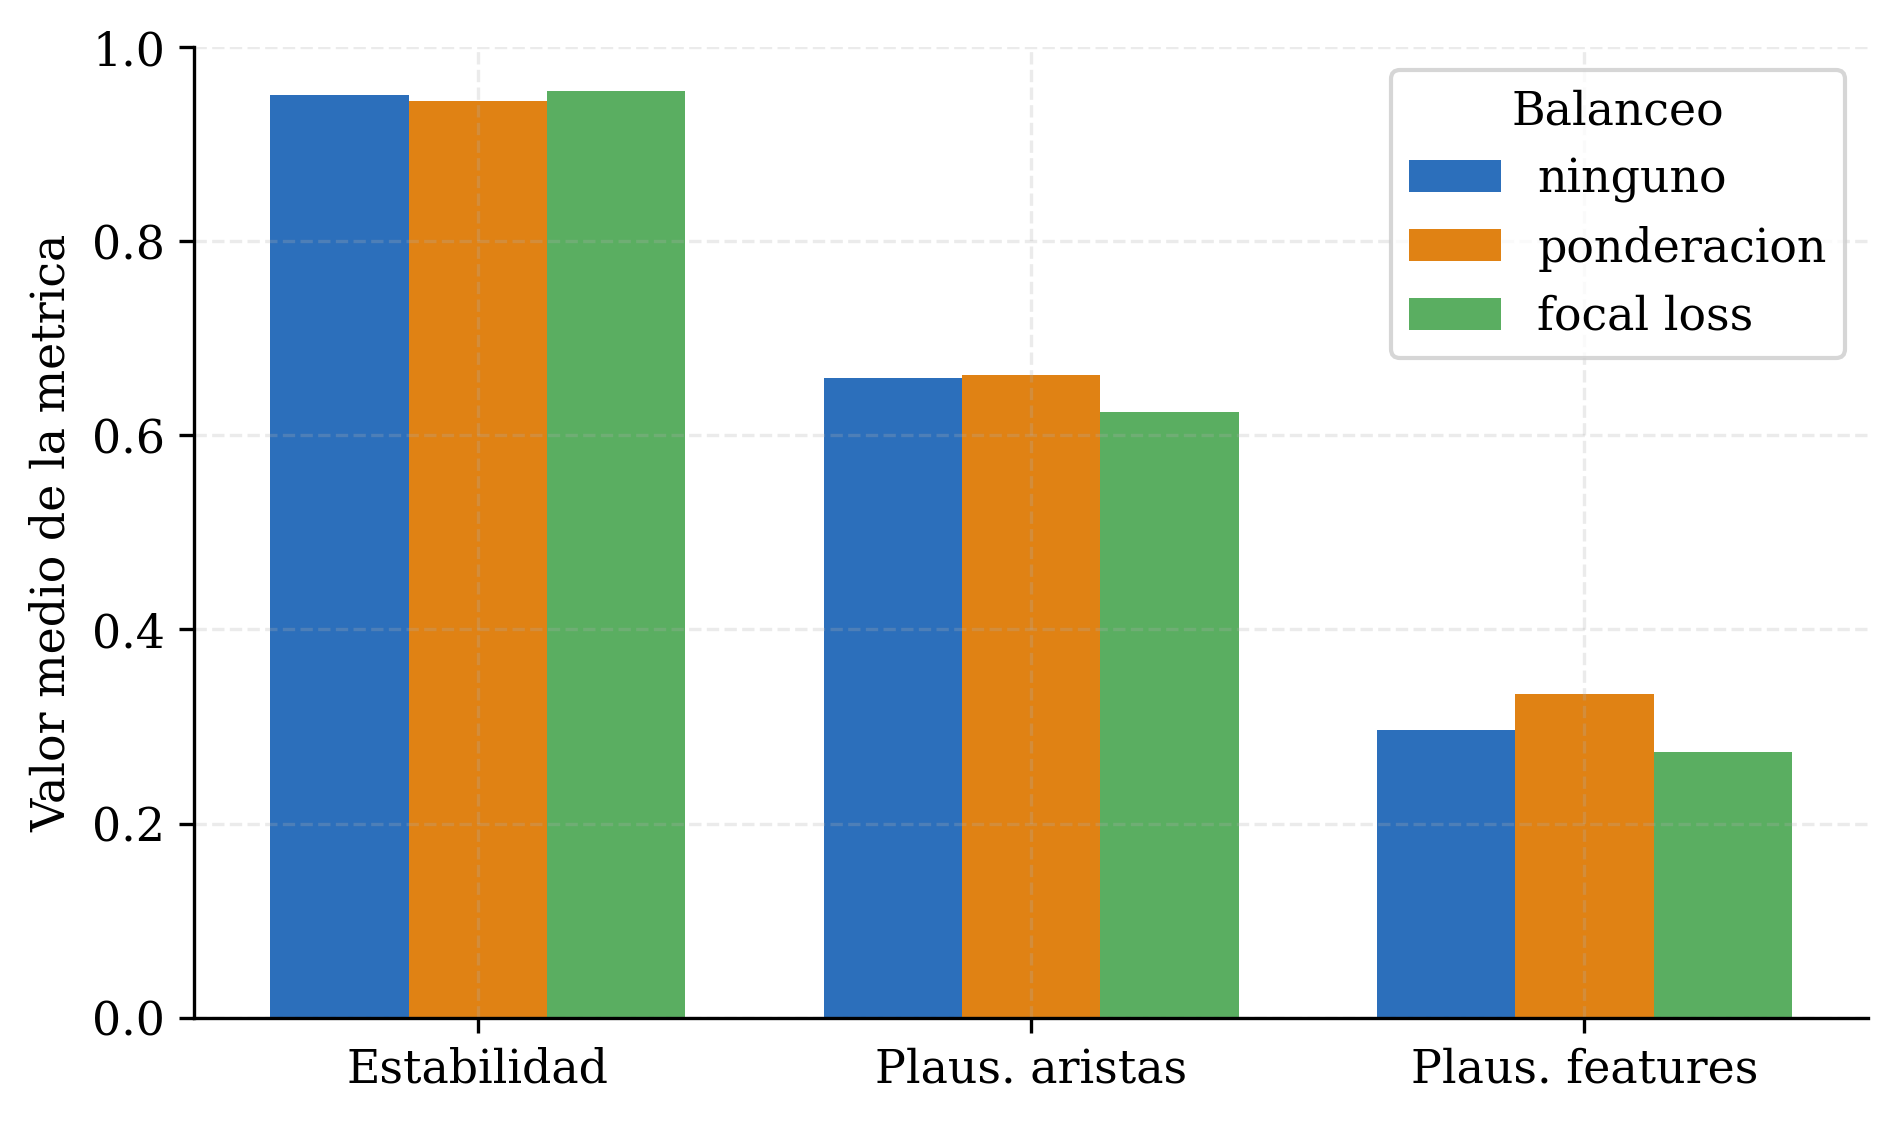
\includegraphics[width=0.85\textwidth]{chapter_5/images_ch5/balanceo_irrelevante.png}
    \caption{Estabilidad y plausibilidad medias por estrategia de balanceo sobre el grafo sintético. Las tres estrategias producen valores prácticamente indistinguibles, lo que confirma que el balanceo apenas influye en la calidad de las explicaciones.}
    \label{fig:balanceo}
\end{figure}

Este hallazgo, aunque de signo negativo, es valioso para la práctica del diseño de sistemas de detección. Buena parte del esfuerzo de diseño en escenarios con desbalance se dedica a elegir y ajustar la estrategia de balanceo, bajo la premisa de que dicha elección influye en el comportamiento del modelo y de sus explicaciones. Los resultados indican que, al menos en lo que respecta a la calidad de las explicaciones sobre un grafo con \textit{ground-truth}, esa premisa no se sostiene, y que la ponderación de clases y la Focal Loss producen explicaciones de calidad equivalente a la del entrenamiento sin intervención. La consecuencia práctica es que la estrategia de balanceo puede elegirse en función del rendimiento predictivo, sin temor a degradar de forma apreciable la interpretabilidad del modelo.

\begin{table}[htbp]
\centering
\renewcommand{\arraystretch}{1.3}
\small
\begin{tabular}{ll ccc}
\toprule
\textbf{Métrica} & \textbf{Factor} & \textbf{Kruskal-Wallis H} & \textbf{valor p} & \textbf{$\eta^2$} \\
\midrule
Estabilidad & arquitectura & 91,1 & $<$0,0001 & 0,24 \\
Estabilidad & explicador & 125,6 & $<$0,0001 & 0,36 \\
Estabilidad & balanceo & 9,1 & 0,0107 & 0,01 \\
Estabilidad & escenario & 9,9 & 0,0423 & 0,04 \\
\midrule
Plaus. aristas & arquitectura & 10,5 & 0,0149 & 0,04 \\
Plaus. aristas & explicador & 195,8 & $<$0,0001 & 0,64 \\
Plaus. aristas & balanceo & 2,4 & 0,3081 & 0,01 \\
Plaus. aristas & escenario & 2,6 & 0,6268 & 0,01 \\
\midrule
Plaus. features & arquitectura & 11,3 & 0,0103 & 0,05 \\
Plaus. features & explicador & 176,2 & $<$0,0001 & 0,45 \\
Plaus. features & balanceo & 3,5 & 0,1730 & 0,01 \\
Plaus. features & escenario & 3,0 & 0,5660 & 0,01 \\
\bottomrule
\end{tabular}
\caption{Prueba de Kruskal-Wallis y tamaño de efecto de cada factor sobre cada métrica en el grafo sintético. El estadístico H corresponde a la prueba no paramétrica, que es la que decide la significancia, mientras que el $\eta^2$ es el tamaño de efecto del análisis de varianza sobre los mismos grupos, incluido como medida de magnitud comparable entre factores. El explicador ejerce el efecto dominante en las tres métricas, la arquitectura solo en la estabilidad, y tanto el balanceo como el escenario de desbalance resultan despreciables.}
\label{tab:synth-stats}
\end{table}


El hallazgo central del eje sintético es la superioridad de PGExplainer sobre GNNExplainer en la plausibilidad de aristas, y la replicación permite comprobar si esa superioridad sobrevive a la variabilidad entre modelos. La comparación se realiza celda por celda mediante la prueba de Wilcoxon de rangos con signo, sobre 225 parejas formadas por cada combinación de grafo, arquitectura, escenario, balanceo y semilla. La diferencia media a favor de PGExplainer es de 0,299 y resulta positiva en el noventa y dos por ciento de las parejas, con un valor de significancia de 2,6 por diez elevado a menos treinta y cinco, como ilustra la Figura \ref{fig:estrella}. La superioridad se mantiene en los tres grafos generados, con valores de plausibilidad de aristas de PGExplainer de 0,820, 0,765 y 0,829, siempre por encima de los valores de GNNExplainer, según recoge la Tabla \ref{tab:grafos}. Este hallazgo, por tanto, no es un artefacto de un único entrenamiento ni de una única realización del grafo, sino un efecto sostenido y estadísticamente sólido.

Conviene preguntarse por qué PGExplainer recupera el patrón de la tipología mejor que GNNExplainer sobre el grafo denso. Una explicación plausible reside en la naturaleza amortizada de PGExplainer, que aprende un modelo paramétrico sobre todo el grafo y, por tanto, captura regularidades compartidas entre los subgrafos de una misma tipología, en lugar de optimizar una máscara de forma aislada para cada nodo. Al aprender de muchos ejemplos, el modelo paramétrico identifica qué configuraciones de aristas son características del patrón, lo que le permite señalar las aristas de la tipología con mayor precisión. GNNExplainer, en cambio, al optimizar cada explicación por separado, carece de esta capacidad de generalización entre nodos, lo que podría explicar su menor plausibilidad de aristas. Esta interpretación es coherente con el hecho de que la ventaja de PGExplainer se sostenga a través de escenarios y de grafos, ya que refleja una propiedad estructural del método y no una casualidad de una configuración particular.

La robustez del hallazgo a través de los escenarios de desbalance queda ilustrada en la Figura \ref{fig:plaus-esc}, que muestra la plausibilidad de aristas de ambos explicadores a lo largo de los cinco escenarios. La ventaja de PGExplainer se mantiene prácticamente constante con independencia del nivel de desbalance, lo que confirma que su superioridad no es un efecto de una proporción de clases particular, sino una propiedad estable del método sobre el grafo denso. Este comportamiento contrasta con la intuición inicial de que el desbalance degradaría la calidad de las explicaciones, y refuerza la conclusión de que el explicador, y no el escenario de desbalance, es el factor determinante de la plausibilidad.

\begin{figure}[htbp]
    \centering
    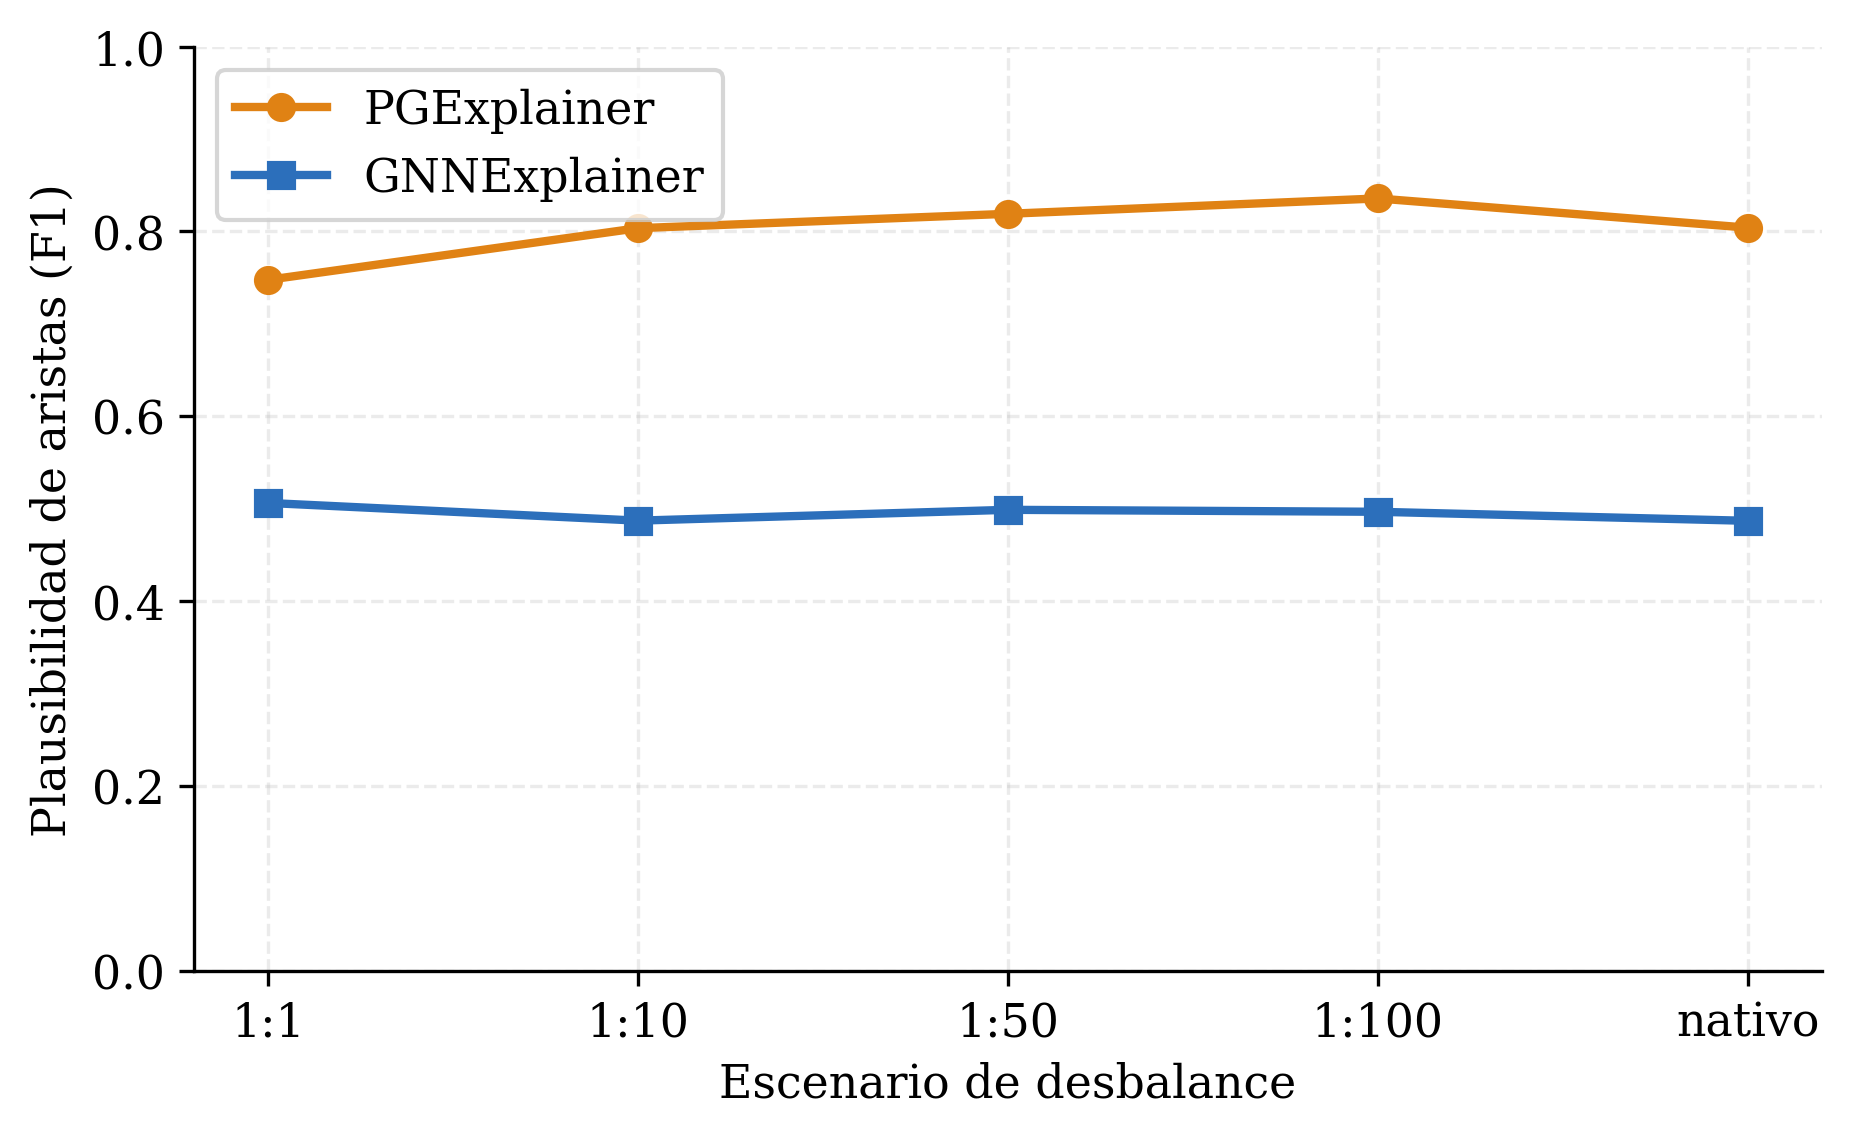
\includegraphics[width=0.8\textwidth]{chapter_5/images_ch5/plaus_escenario.png}
    \caption{Plausibilidad de aristas de PGExplainer y GNNExplainer a lo largo de los cinco escenarios de desbalance sobre el grafo sintético. La ventaja de PGExplainer se mantiene constante con independencia del nivel de desbalance, lo que confirma la robustez del hallazgo frente a la proporción de clases.}
    \label{fig:plaus-esc}
\end{figure}

\begin{figure}[htbp]
    \centering
    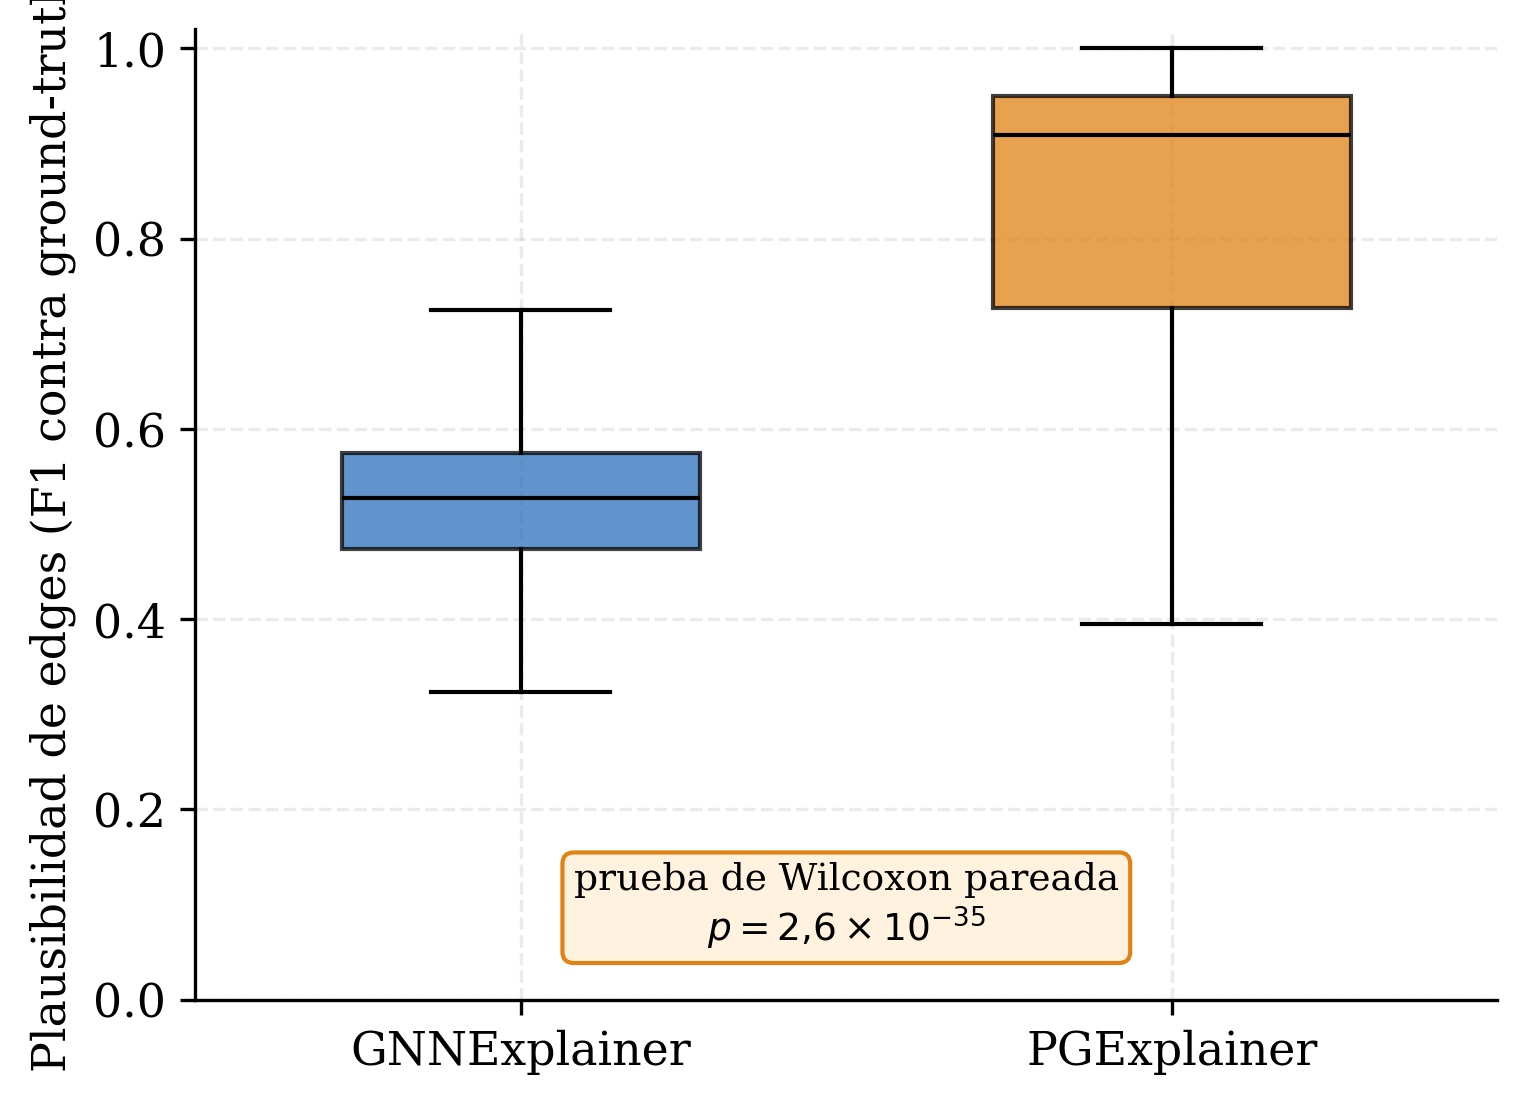
\includegraphics[width=0.6\textwidth]{chapter_5/images_ch5/hallazgo_estrella.png}
    \caption{Distribución de la plausibilidad de aristas por explicador sobre el grafo sintético. PGExplainer recupera las aristas de la tipología con una plausibilidad claramente superior a la de GNNExplainer, una diferencia confirmada por la prueba de Wilcoxon pareada.}
    \label{fig:estrella}
\end{figure}

\begin{table}[htbp]
    \centering
    \renewcommand{\arraystretch}{1.3}
    \begin{tabular}{lccc}
    \toprule
    \textbf{Explicador} & \textbf{Grafo 0} & \textbf{Grafo 1} & \textbf{Grafo 2} \\
    \midrule
    PGExplainer  & 0,801 & 0,765 & 0,829 \\
    GNNExplainer & 0,495 & 0,523 & 0,529 \\
    \bottomrule
    \end{tabular}
    \caption{Plausibilidad de aristas de PGExplainer y GNNExplainer en las tres realizaciones del grafo sintético. La superioridad de PGExplainer se mantiene en las tres instancias, lo que confirma que el hallazgo no depende de una realización particular.}
    \label{tab:grafos}
\end{table}

\section{La Ausencia de un Puente entre Estabilidad y Plausibilidad}

Una hipótesis natural, presente de forma implícita en buena parte de la literatura, sostiene que una explicación más estable debería ser también más plausible, bajo la intuición de que la consistencia entre ejecuciones reflejaría un acierto sobre el patrón real. El eje sintético permite contrastar esta hipótesis de forma directa, correlacionando la estabilidad de cada explicación con su plausibilidad, y el resultado es un puente nulo. Para GNNExplainer, la correlación entre estabilidad y plausibilidad de features es de -0,014, con un intervalo de confianza al noventa y cinco por ciento que va de -0,038 a 0,011 y que, por tanto, incluye el cero, como muestra la Figura \ref{fig:puente}. Para GNNShap, la correlación es de 0,034 con un intervalo de 0,013 a 0,053, distinguible del cero solo por el tamaño de la muestra y de una magnitud tan pequeña que carece de significado práctico, ya que explica alrededor del uno por mil de la variabilidad.

\begin{figure}[htbp]
    \centering
    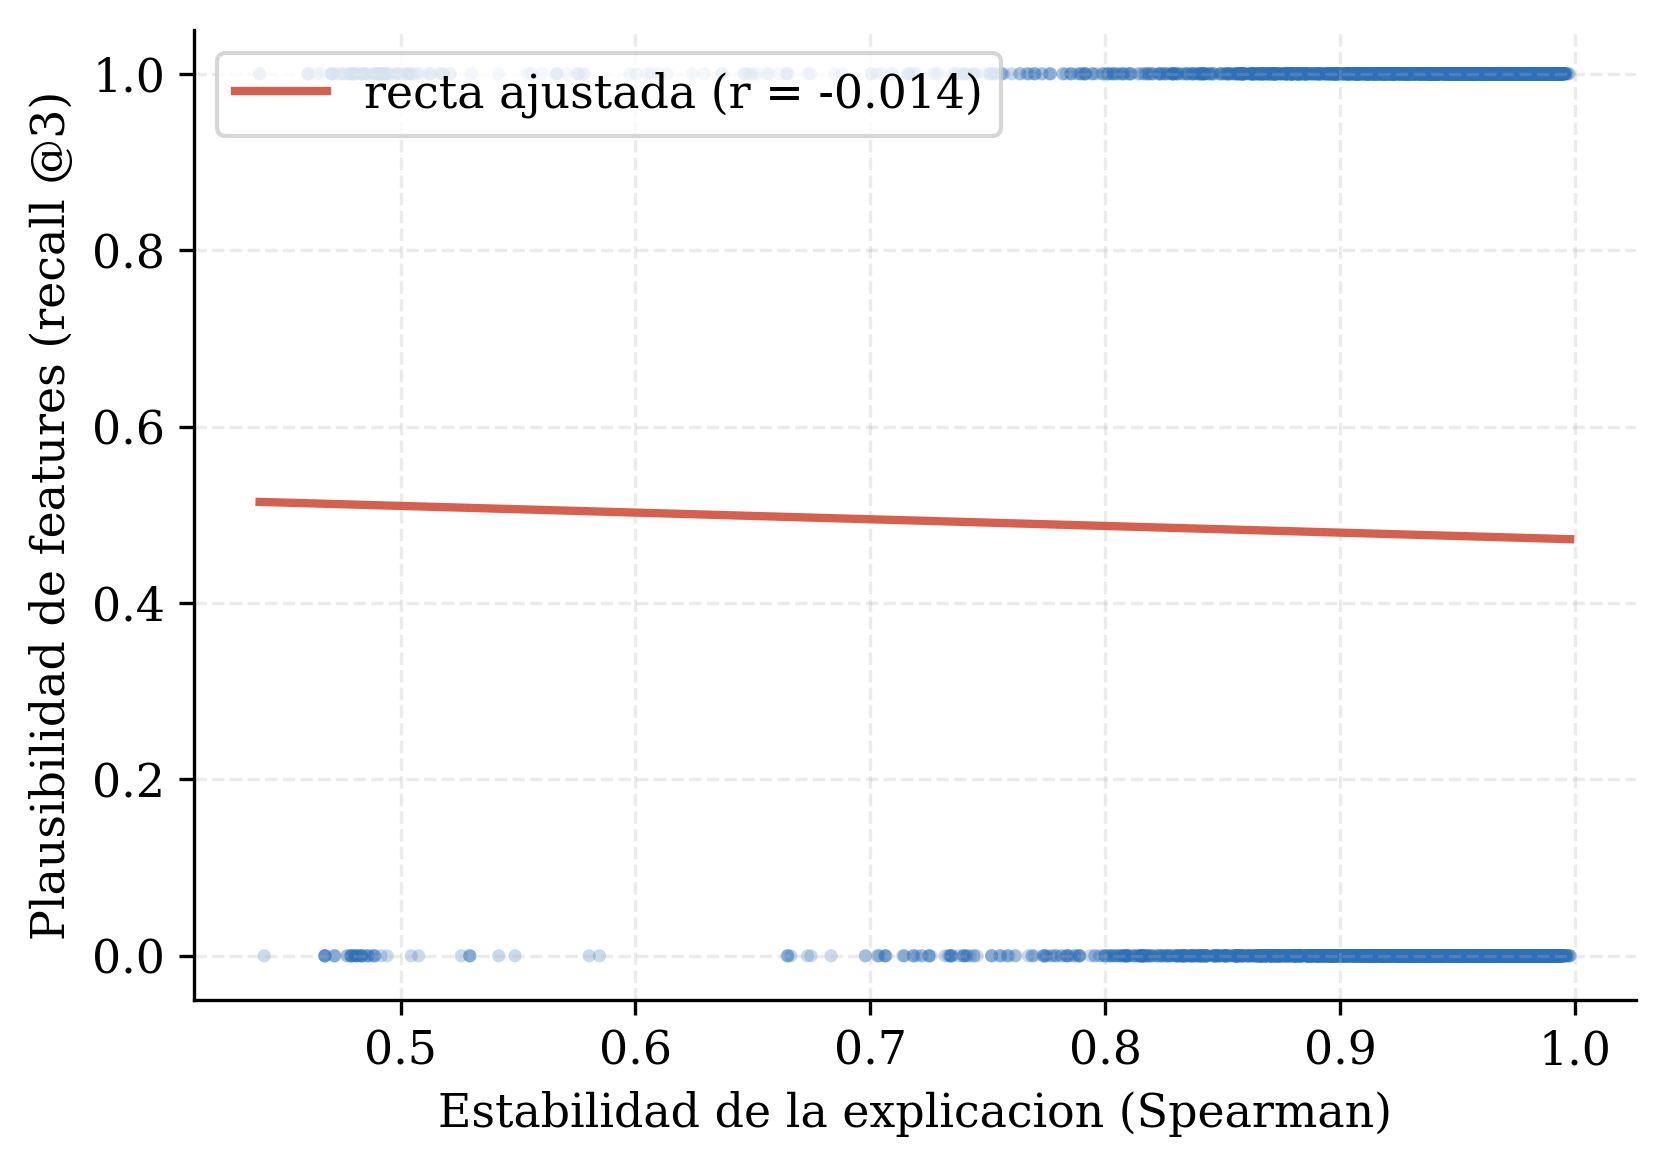
\includegraphics[width=0.7\textwidth]{chapter_5/images_ch5/puente_nulo.png}
    \caption{Relación entre la estabilidad de las explicaciones y su plausibilidad de features para GNNExplainer sobre el grafo sintético. La recta ajustada es prácticamente plana y la correlación de -0,014 no se distingue de cero, lo que evidencia la ausencia de una ley que ligue estabilidad con plausibilidad.}
    \label{fig:puente}
\end{figure}

El análisis por tipología confirma que no existe una ley universal que ligue ambas dimensiones, ya que el signo de la relación cambia según la tipología considerada. En las tipologías \textit{structuring} y \textit{fan-out} la correlación entre estabilidad y plausibilidad de aristas es positiva, con valores de 0,344 y 0,307, mientras que en \textit{layering} es negativa, con un valor de -0,102, y en \textit{fan-in} resulta nula, tal como presenta la Tabla \ref{tab:synth-bridge} junto con los intervalos de confianza bootstrap.

\begin{table}[htbp]
\centering
\renewcommand{\arraystretch}{1.3}
\begin{tabular}{lcc}
\toprule
\textbf{Tipologia} & \textbf{r (estab., aristas)} & \textbf{IC 95\%} \\
\midrule
STRUCTURING & +0,344 & [+0,301, +0,386] \\
LAYERING & -0,102 & [-0,146, -0,055] \\
FAN\_IN & -0,044 & [-0,105, +0,020] \\
FAN\_OUT & +0,307 & [+0,247, +0,362] \\
\bottomrule
\end{tabular}
\caption{Correlacion entre estabilidad y plausibilidad de aristas por tipologia para GNNExplainer, con intervalo de confianza bootstrap. El signo cambia entre tipologias, lo que confirma la ausencia de una ley universal.}
\label{tab:synth-bridge}
\end{table}
 Esta heterogeneidad, junto con el valor global cercano a cero, sostiene una conclusión clara, un explicador estable no es por ello más plausible, y ambas propiedades deben medirse por separado. Esta conclusión es coherente con las corridas previas del eje sintético, que ya habían encontrado un puente débil o nulo, y adquiere aquí un respaldo estadístico explícito mediante intervalos de confianza.

\section{La Disociación entre Plausibilidad y Fidelidad}

El análisis de la fidelidad, medida de forma uniforme para los tres explicadores, revela una tensión que la matriz factorial de una sola corrida no permitía apreciar y que constituye un hallazgo nuevo de este trabajo. PGExplainer, que es el explicador más plausible en aristas, resulta al mismo tiempo el menos fiel al modelo, con una caída de la probabilidad al retirar sus aristas de apenas 0,07 a 0,13 según la arquitectura. GNNExplainer presenta el comportamiento inverso, ya que es menos plausible pero mucho más fiel, con caídas de 0,52 a 0,63. La Figura \ref{fig:disociacion} contrasta ambas dimensiones y hace visible que la plausibilidad y la fidelidad no solo no coinciden, sino que se ordenan de manera opuesta entre estos dos explicadores.

\begin{figure}[htbp]
    \centering
    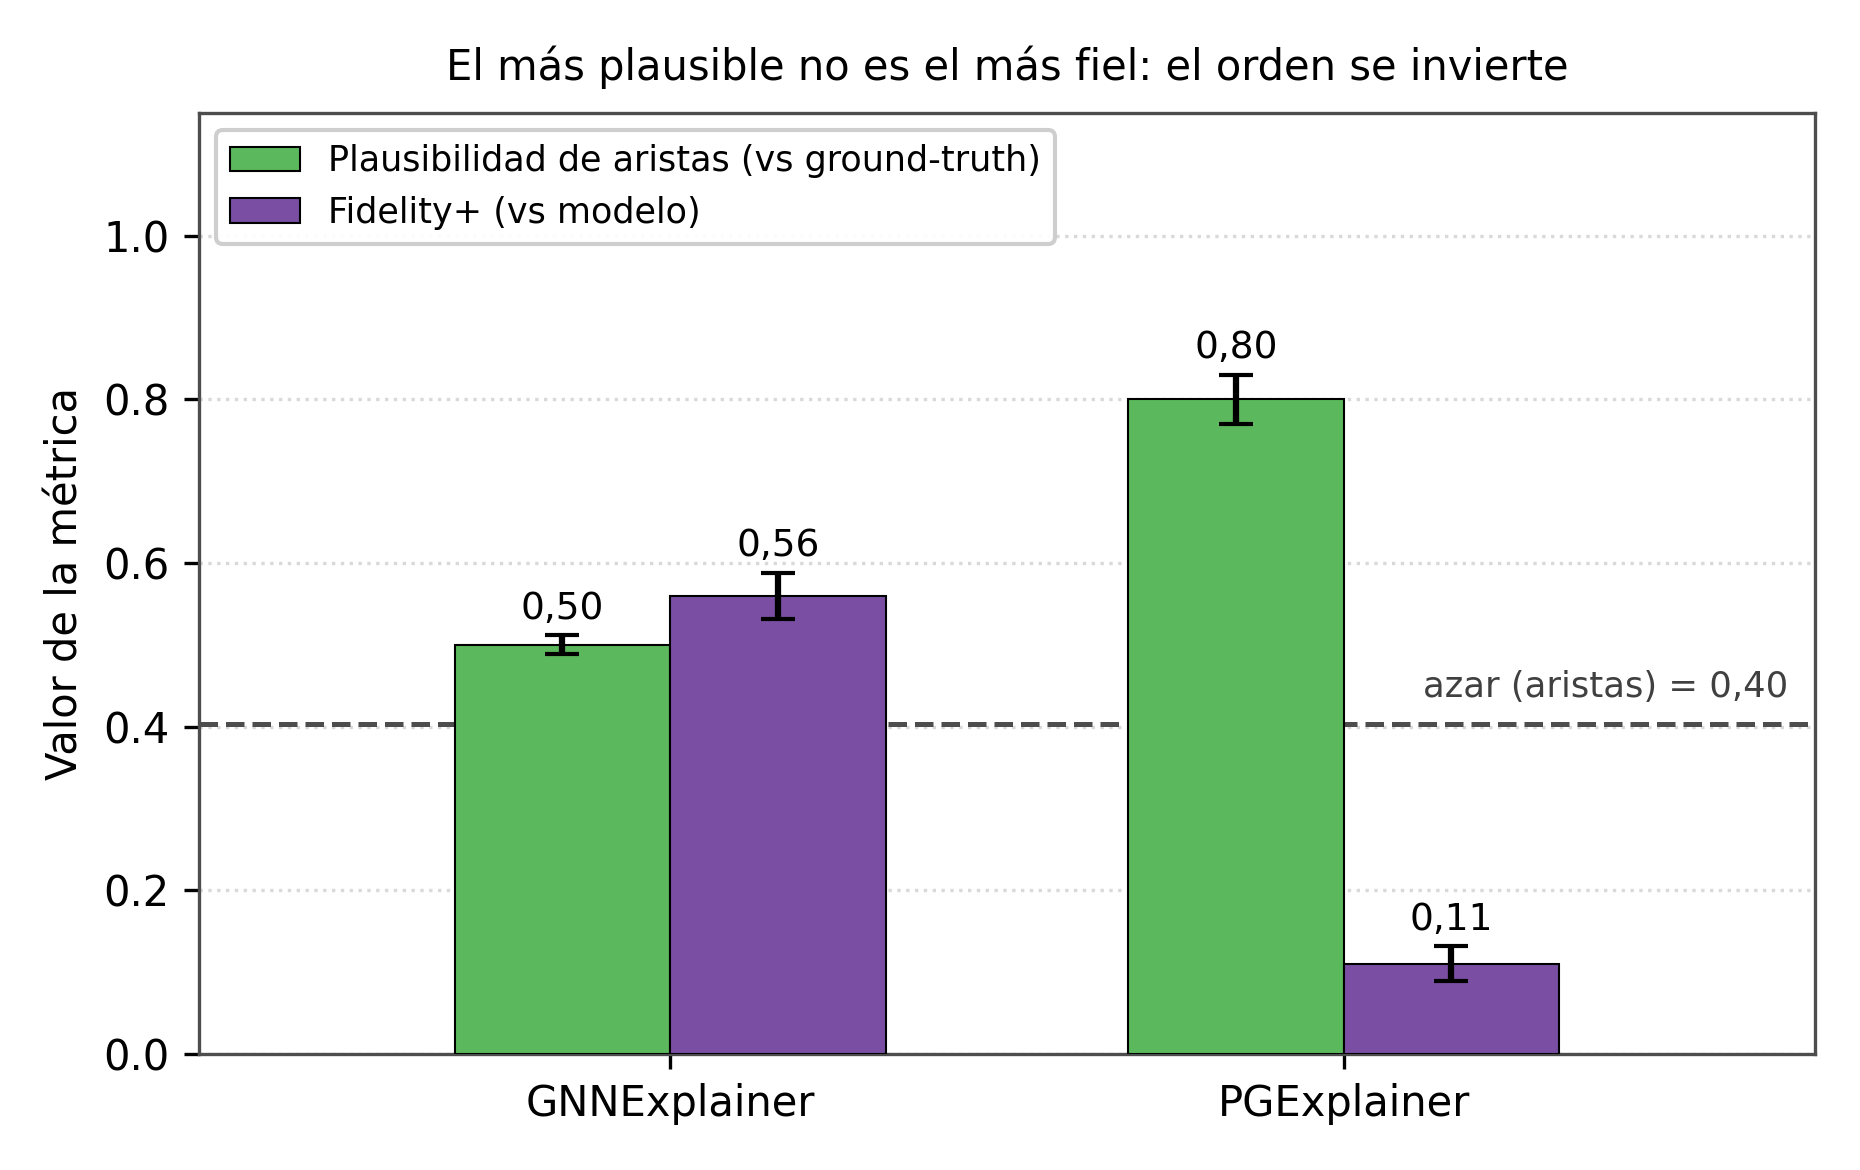
\includegraphics[width=0.85\textwidth]{chapter_5/images_ch5/disociacion.png}
    \caption{Plausibilidad frente a fidelidad positiva por explicador sobre el grafo sintético. PGExplainer es el más plausible pero el menos fiel, mientras que GNNExplainer invierte el orden, lo que evidencia la disociación entre lo que resulta plausible para un observador y lo que es fiel al mecanismo del modelo.}
    \label{fig:disociacion}
\end{figure}

La interpretación de esta disociación es a la vez sencilla y profunda. PGExplainer recupera las aristas que definen el patrón de lavado según el \textit{ground-truth}, es decir aquellas que un analista humano reconocería como la tipología, mientras que GNNExplainer recupera las aristas que el modelo realmente utiliza para decidir, y ambos conjuntos no coinciden. Dicho de otro modo, una explicación puede ser plausible, en el sentido de alinearse con el patrón que un humano considera correcto, sin ser fiel, en el sentido de reflejar el mecanismo interno del modelo, y viceversa. Esta tensión entre plausibilidad y fidelidad es un concepto conocido en la teoría de la explicabilidad, pero solo un régimen sintético con \textit{ground-truth} de tipología permite exhibirla de forma cuantitativa, ya que requiere medir simultáneamente ambas dimensiones sobre las mismas explicaciones, algo imposible en un dataset sin patrón de referencia.

La disociación tiene además una lectura práctica para quien debe elegir un explicador. Si el objetivo de una auditoría es convencer a un revisor humano de que una alerta corresponde a un patrón de lavado conocido, la plausibilidad es la propiedad relevante, y PGExplainer resulta el más adecuado pese a su baja fidelidad. Si, en cambio, el objetivo es certificar en qué se basa realmente el modelo, para detectar por ejemplo si depende de una característica espuria, la fidelidad es la propiedad relevante, y GNNExplainer resulta preferible pese a su menor plausibilidad. La imposibilidad de optimizar ambas dimensiones a la vez convierte la elección del explicador en una decisión que depende del propósito, y no en una cuestión con una única respuesta correcta. Este matiz, que la disociación hace visible, rara vez se plantea en la literatura de explicabilidad, que tiende a buscar el mejor método en abstracto.

La Figura \ref{fig:fid-arq} desglosa la fidelidad positiva por arquitectura y explicador, y confirma que el patrón de la disociación se mantiene a través de las cuatro arquitecturas. GNNExplainer conserva la fidelidad más alta en todas ellas, mientras que PGExplainer permanece en la parte baja con independencia de la arquitectura, lo que refuerza que la disociación es una propiedad del explicador y no un efecto de una arquitectura concreta.

\begin{figure}[htbp]
    \centering
    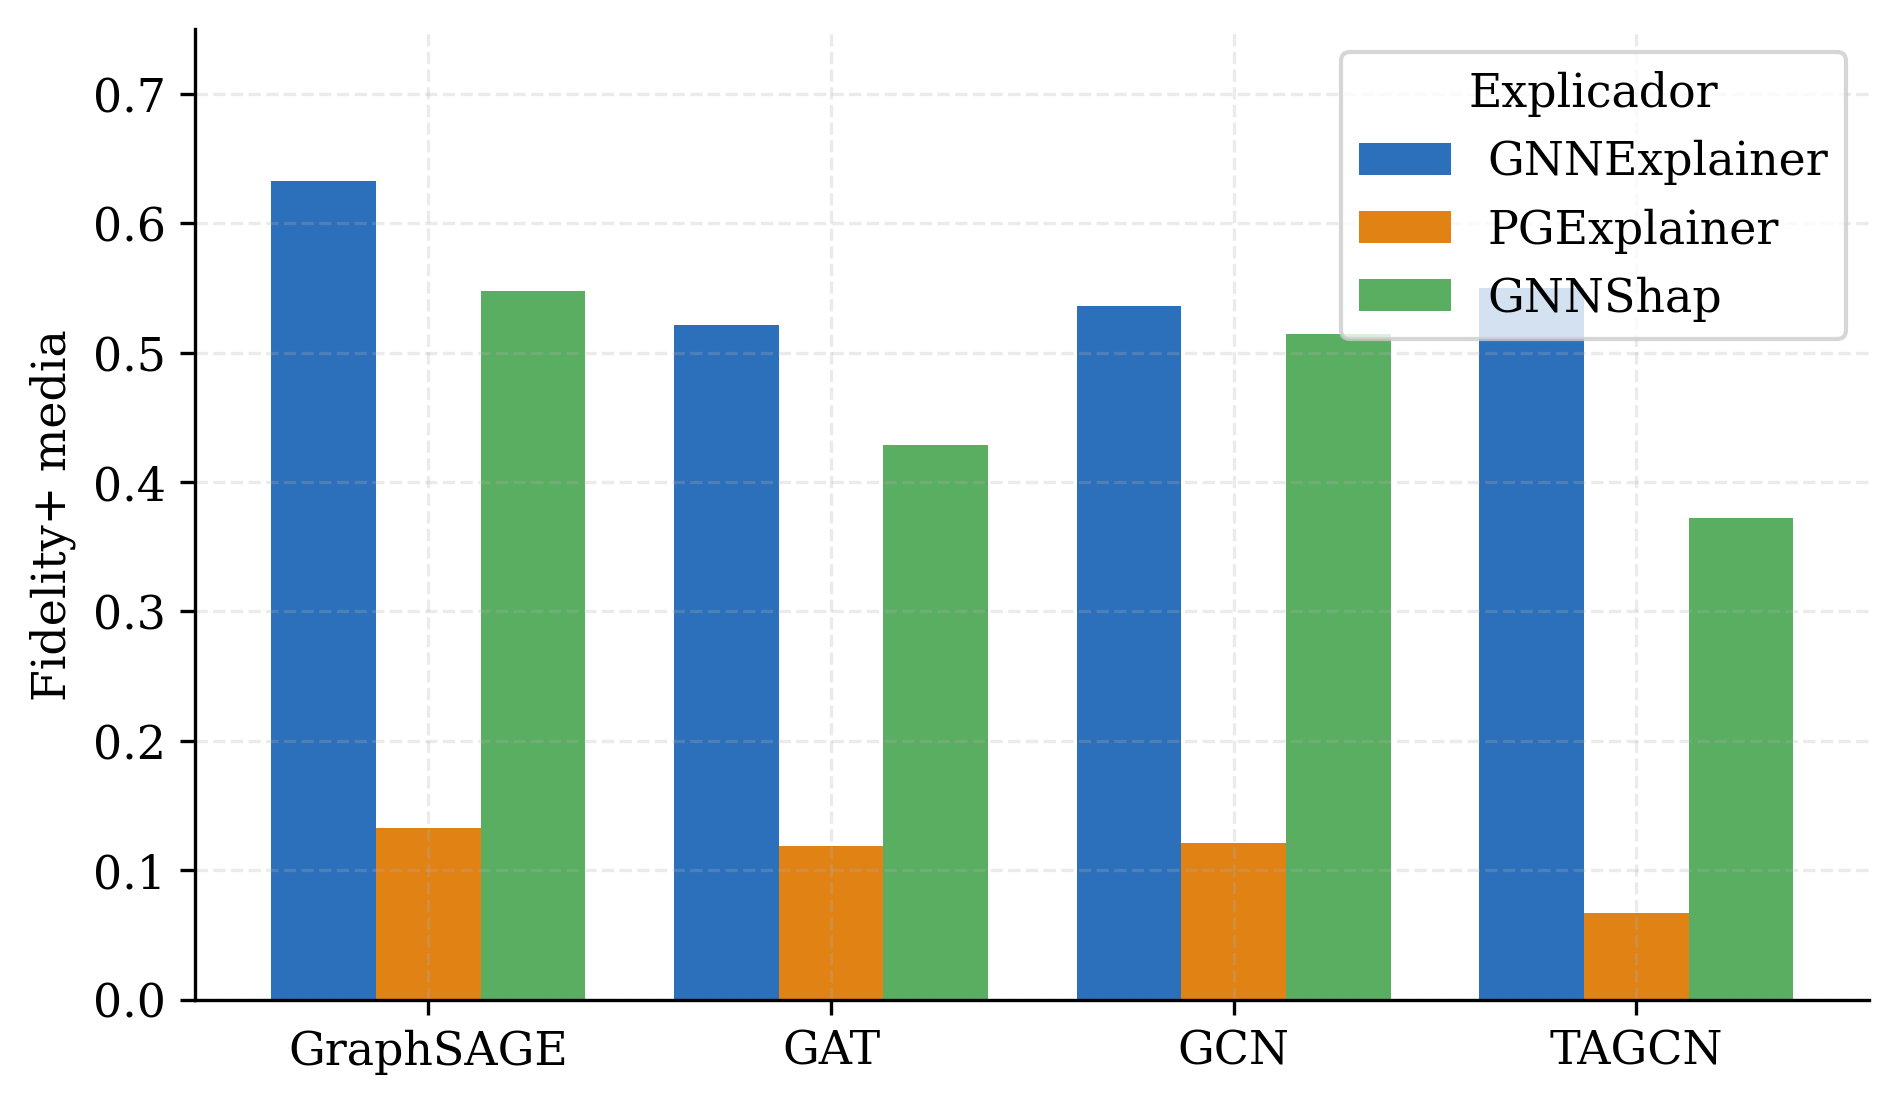
\includegraphics[width=0.85\textwidth]{chapter_5/images_ch5/fidelidad_arq.png}
    \caption{Fidelity+ media por arquitectura y explicador sobre el grafo sintético. GNNExplainer mantiene la mayor fidelidad en las cuatro arquitecturas y PGExplainer la menor, lo que confirma que la disociación entre plausibilidad y fidelidad es una propiedad del explicador y no de una arquitectura concreta.}
    \label{fig:fid-arq}
\end{figure}

\section{Síntesis del Eje Sintético}

El eje sintético cumple el propósito que motivó su construcción, medir aquello que el \textit{Elliptic Dataset} no permite y sostenerlo con un análisis estadístico riguroso. Los resultados dejan tres conclusiones que estructuran la discusión del capítulo siguiente. La primera es que el explicador es el factor determinante de la calidad de las explicaciones, muy por encima de la arquitectura y del balanceo, y que PGExplainer supera a GNNExplainer en plausibilidad de aristas de forma robusta a la variabilidad entre modelos y entre grafos. La segunda es que no existe un puente entre estabilidad y plausibilidad, de modo que un explicador estable no es por ello más acertado sobre el patrón real. La tercera es la disociación entre plausibilidad y fidelidad, que obliga a distinguir con cuidado entre una explicación que convence a un humano y una explicación que refleja el razonamiento del modelo. Más allá de estos tres hallazgos, el eje sintético demuestra la viabilidad de un enfoque de evaluación que la comunidad de explicabilidad podría adoptar de forma más amplia. Al construir un grafo con \textit{ground-truth} de tipología y densidad controlada, se obtiene un banco de pruebas en el que la plausibilidad, la fidelidad y la estabilidad de un explicador pueden medirse de forma simultánea y objetiva, algo que los conjuntos de datos reales rara vez permiten. Este enfoque no sustituye la validación sobre datos reales, pero la complementa al ofrecer un entorno en el que las afirmaciones sobre la calidad de una explicación son verificables contra una referencia conocida. La combinación de ambos tipos de evidencia, la validez externa de los datos reales y la validez interna del grafo controlado, es lo que confiere solidez a las conclusiones de esta tesis.

Estas conclusiones, junto con las del eje Elliptic, se integran y se discuten en el Capítulo 6.
